\documentclass[tikz]{standalone}
\usepackage{amsmath,amssymb}
\usetikzlibrary{arrows.meta}

% Classes of morphisms
\newcommand{\all}{\mathsf{all}}
\newcommand{\inj}{\mathsf{inj}}
\newcommand{\surj}{\mathsf{surj}}
\newcommand{\bij}{\mathsf{bij}}
\newcommand{\init}{\mathsf{init}}
\newcommand{\pb}{\mathsf{pb}}
\newcommand{\homog}{\mathsf{homog}}
\DeclareMathOperator{\id}{id}
\begin{document}
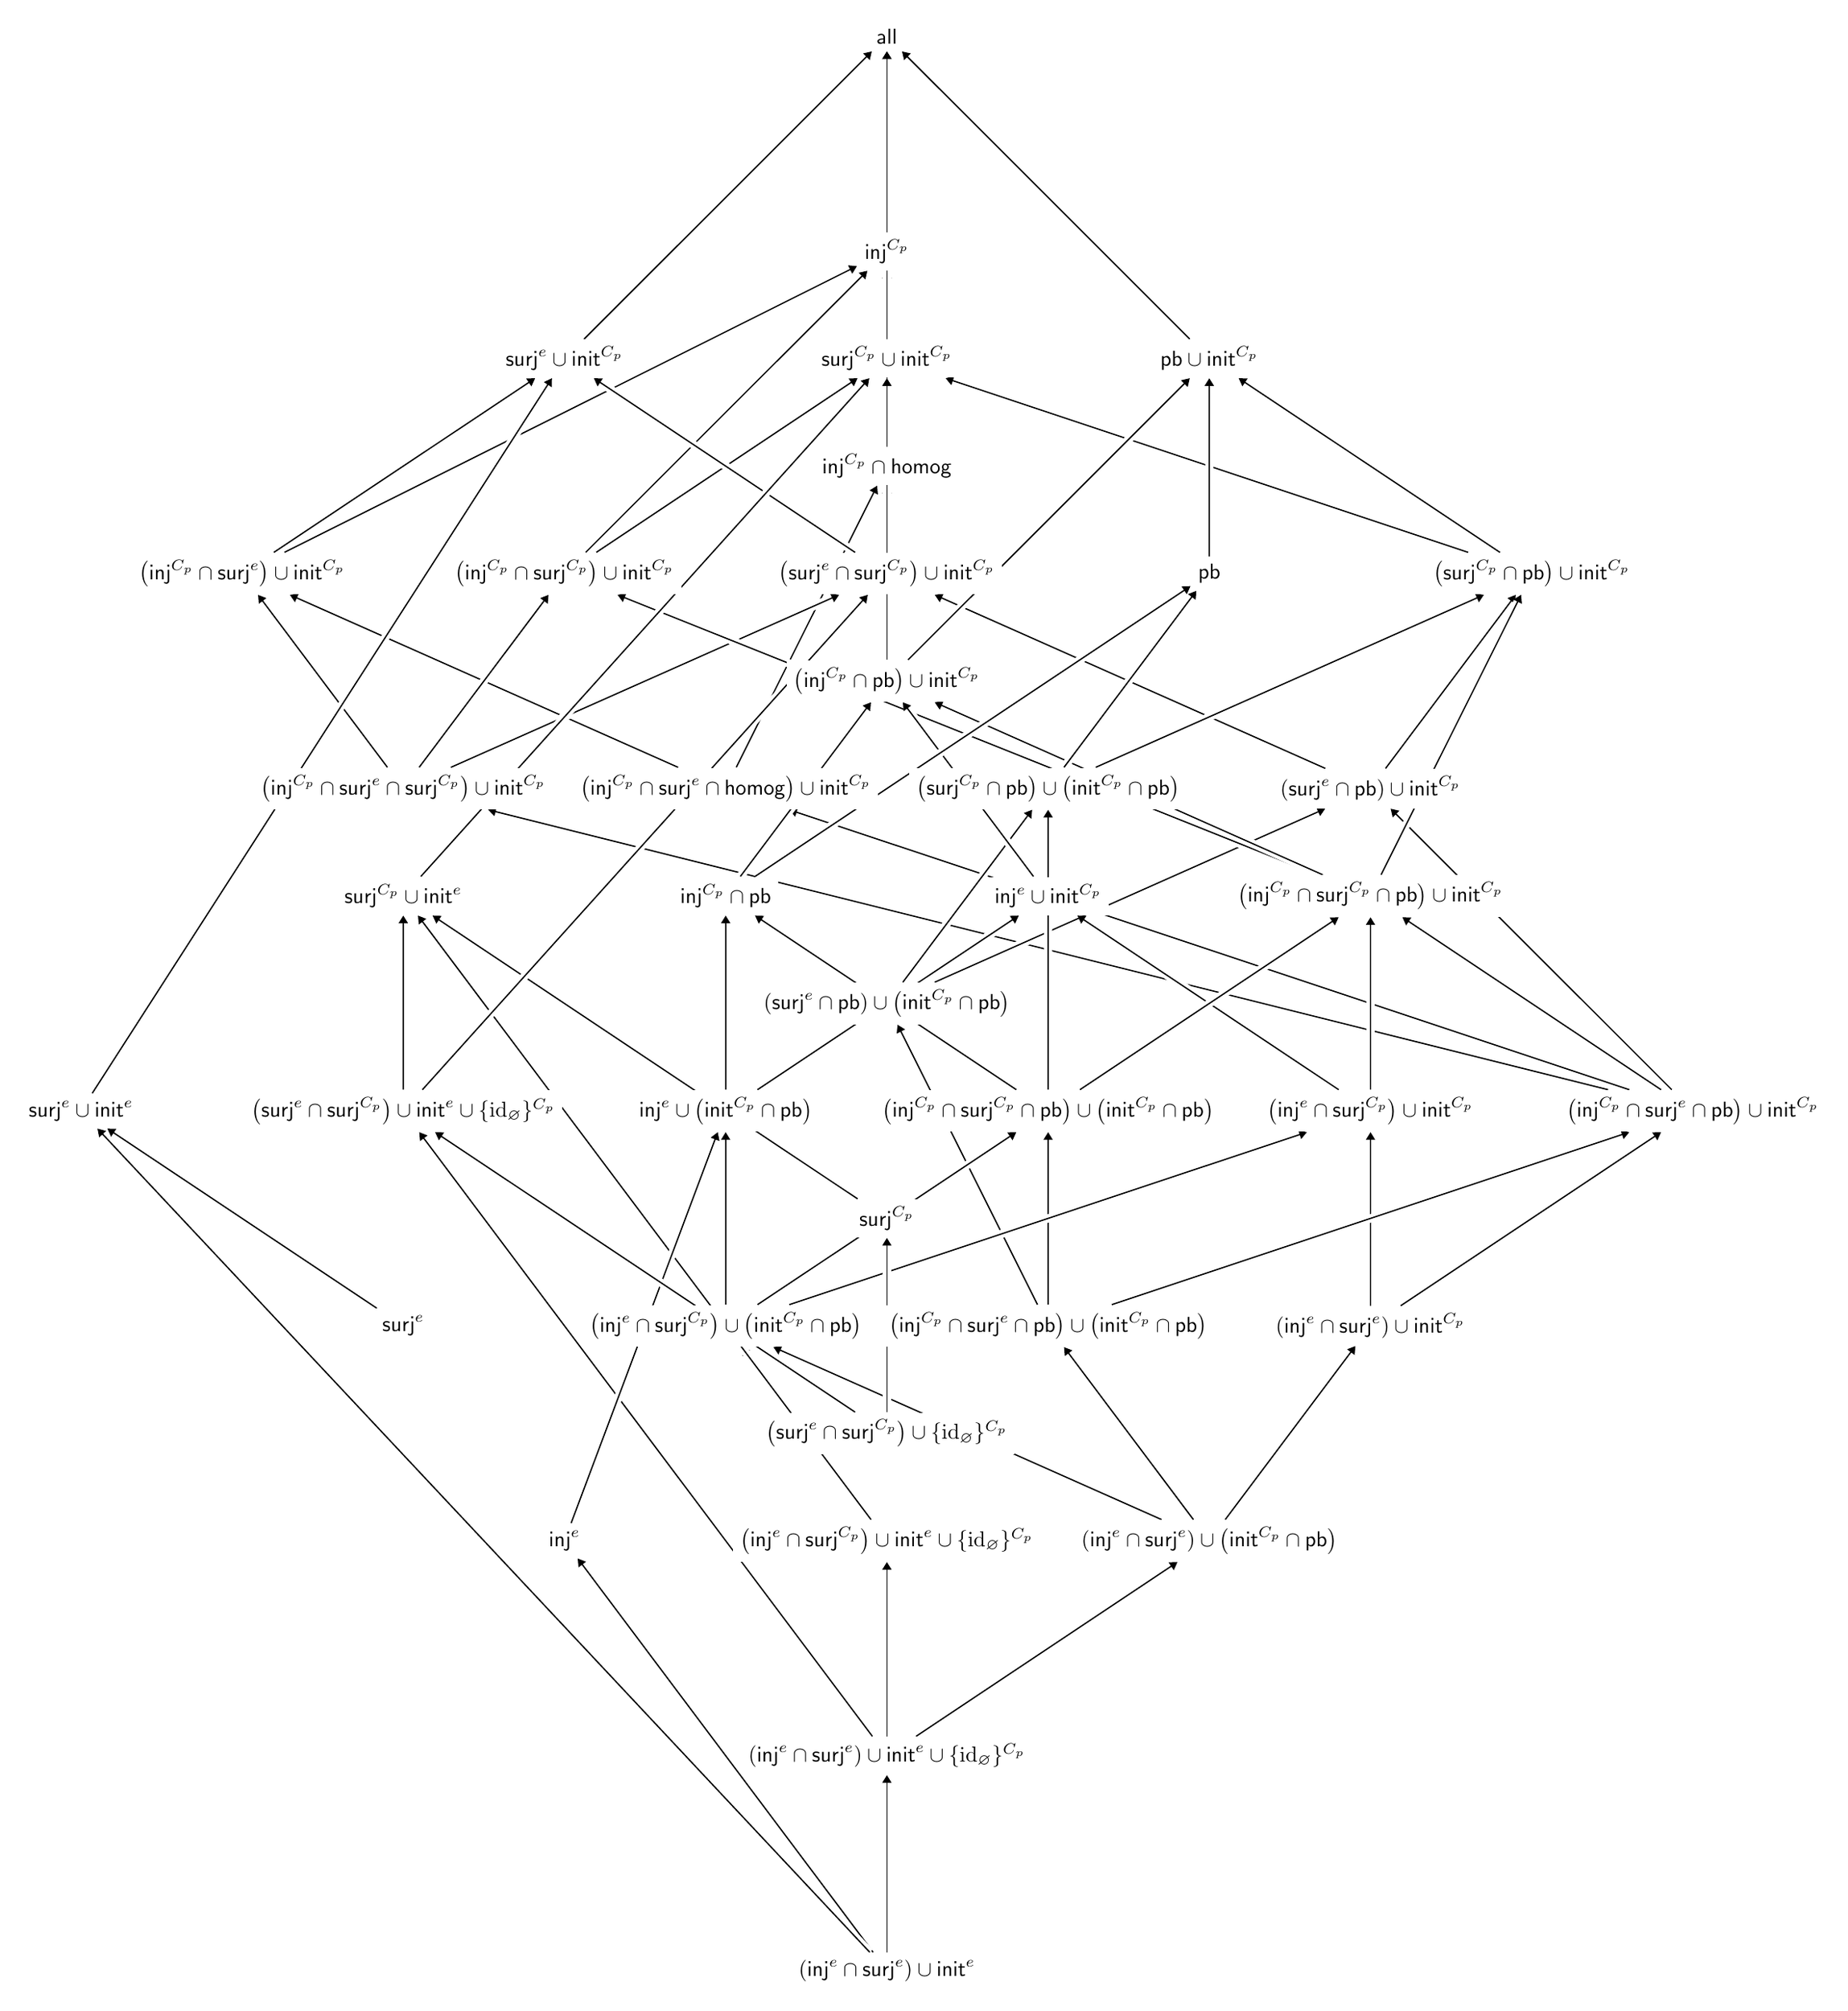
\begin{tikzpicture}[scale=3.5]
\node (v0) at (0, 4.5) {$ \all $};
\node (v1) at (0, 3.5) {$ \inj^{C_p} $};
\node (v2) at (-2.25, -1.5) {$ \surj^e $};
\node (v3) at (-3.75, -0.5) {$ \surj^e \cup \init^e $};
\node (v4) at (-1.5, 3) {$ \surj^e \cup \init^{C_p} $};
\node (v5) at (0, -1) {$ \surj^{C_p} $};
\node (v6) at (-2.25, 0.5) {$ \surj^{C_p} \cup \init^e $};
\node (v7) at (0, 3) {$ \surj^{C_p} \cup \init^{C_p} $};
\node (v8) at (-3, 2) {$ \left(\inj^{C_p} \cap \surj^e\right) \cup \init^{C_p} $};
\node (v9) at (-1.5, 2) {$ \left(\inj^{C_p} \cap \surj^{C_p}\right) \cup \init^{C_p} $};
\node (v10) at (0, 2.5) {$ \inj^{C_p} \cap \homog $};
\node (v11) at (0, -2) {$ \left(\surj^e \cap \surj^{C_p}\right) \cup \{\id_\varnothing\}^{C_p} $};
\node (v12) at (-2.25, -0.5) {$ \left(\surj^e \cap \surj^{C_p}\right) \cup \init^e \cup \{\id_\varnothing\}^{C_p} $};
\node (v13) at (0, 2) {$ \left(\surj^e \cap \surj^{C_p}\right) \cup \init^{C_p} $};
\node (v14) at (1.5, 2) {$ \pb $};
\node (v15) at (1.5, 3) {$ \pb \cup \init^{C_p} $};
\node (v16) at (-2.25, 1) {$ \left(\inj^{C_p} \cap \surj^e \cap \surj^{C_p}\right) \cup \init^{C_p} $};
\node (v17) at (-0.75, 1) {$ \left(\inj^{C_p} \cap \surj^e \cap \homog\right) \cup \init^{C_p} $};
\node (v18) at (-0.75, 0.5) {$ \inj^{C_p} \cap \pb $};
\node (v19) at (0, 1.5) {$ \left(\inj^{C_p} \cap \pb\right) \cup \init^{C_p} $};
\node (v20) at (0.75, 1) {$ \left(\surj^{C_p} \cap \pb\right) \cup \left(\init^{C_p} \cap \pb\right) $};
\node (v21) at (3, 2) {$ \left(\surj^{C_p} \cap \pb\right) \cup \init^{C_p} $};
\node (v22) at (-1.5, -2.5) {$ \inj^e $};
\node (v23) at (-0.75, -0.5) {$ \inj^e \cup \left(\init^{C_p} \cap \pb\right) $};
\node (v24) at (0.75, 0.5) {$ \inj^e \cup \init^{C_p} $};
\node (v25) at (0.75, -0.5) {$ \left(\inj^{C_p} \cap \surj^{C_p} \cap \pb\right) \cup \left(\init^{C_p} \cap \pb\right) $};
\node (v26) at (2.25, 0.5) {$ \left(\inj^{C_p} \cap \surj^{C_p} \cap \pb\right) \cup \init^{C_p} $};
\node (v27) at (0, 0) {$ \left(\surj^e \cap \pb\right) \cup \left(\init^{C_p} \cap \pb\right) $};
\node (v28) at (2.25, 1) {$ \left(\surj^e \cap \pb\right) \cup \init^{C_p} $};
\node (v29) at (0, -2.5) {$ \left(\inj^e \cap \surj^{C_p}\right) \cup \init^e \cup \{\id_\varnothing\}^{C_p} $};
\node (v30) at (-0.75, -1.5) {$ \left(\inj^e \cap \surj^{C_p}\right) \cup \left(\init^{C_p} \cap \pb\right) $};
\node (v31) at (2.25, -0.5) {$ \left(\inj^e \cap \surj^{C_p}\right) \cup \init^{C_p} $};
\node (v32) at (0.75, -1.5) {$ \left(\inj^{C_p} \cap \surj^e \cap \pb\right) \cup \left(\init^{C_p} \cap \pb\right) $};
\node (v33) at (3.75, -0.5) {$ \left(\inj^{C_p} \cap \surj^e \cap \pb\right) \cup \init^{C_p} $};
\node (v34) at (0, -4.5) {$ \left(\inj^e \cap \surj^e\right) \cup \init^e $};
\node (v35) at (0, -3.5) {$ \left(\inj^e \cap \surj^e\right) \cup \init^e \cup \{\id_\varnothing\}^{C_p} $};
\node (v36) at (1.5, -2.5) {$ \left(\inj^e \cap \surj^e\right) \cup \left(\init^{C_p} \cap \pb\right) $};
\node (v37) at (2.25, -1.5) {$ \left(\inj^e \cap \surj^e\right) \cup \init^{C_p} $};
\draw[white, ultra thick, double=black, arrows={-Triangle[black,scale=0.25]}] (v34) -- (v35);
\draw[white, ultra thick, double=black, arrows={-Triangle[black,scale=0.25]}] (v34) -- (v22);
\draw[white, ultra thick, double=black, arrows={-Triangle[black,scale=0.25]}] (v34) -- (v3);
\draw[white, ultra thick, double=black, arrows={-Triangle[black,scale=0.25]}] (v35) -- (v36);
\draw[white, ultra thick, double=black, arrows={-Triangle[black,scale=0.25]}] (v35) -- (v29);
\draw[white, ultra thick, double=black, arrows={-Triangle[black,scale=0.25]}] (v35) -- (v12);
\draw[white, ultra thick, double=black, arrows={-Triangle[black,scale=0.25]}] (v36) -- (v37);
\draw[white, ultra thick, double=black, arrows={-Triangle[black,scale=0.25]}] (v36) -- (v32);
\draw[white, ultra thick, double=black, arrows={-Triangle[black,scale=0.25]}] (v36) -- (v30);
\draw[white, ultra thick, double=black, arrows={-Triangle[black,scale=0.25]}] (v37) -- (v33);
\draw[white, ultra thick, double=black, arrows={-Triangle[black,scale=0.25]}] (v37) -- (v31);
\draw[white, ultra thick, double=black, arrows={-Triangle[black,scale=0.25]}] (v32) -- (v33);
\draw[white, ultra thick, double=black, arrows={-Triangle[black,scale=0.25]}] (v32) -- (v27);
\draw[white, ultra thick, double=black, arrows={-Triangle[black,scale=0.25]}] (v32) -- (v25);
\draw[white, ultra thick, double=black, arrows={-Triangle[black,scale=0.25]}] (v33) -- (v17);
\draw[white, ultra thick, double=black, arrows={-Triangle[black,scale=0.25]}] (v33) -- (v16);
\draw[white, ultra thick, double=black, arrows={-Triangle[black,scale=0.25]}] (v33) -- (v28);
\draw[white, ultra thick, double=black, arrows={-Triangle[black,scale=0.25]}] (v33) -- (v26);
\draw[white, ultra thick, double=black, arrows={-Triangle[black,scale=0.25]}] (v17) -- (v8);
\draw[white, ultra thick, double=black, arrows={-Triangle[black,scale=0.25]}] (v17) -- (v10);
\draw[white, ultra thick, double=black, arrows={-Triangle[black,scale=0.25]}] (v16) -- (v8);
\draw[white, ultra thick, double=black, arrows={-Triangle[black,scale=0.25]}] (v16) -- (v9);
\draw[white, ultra thick, double=black, arrows={-Triangle[black,scale=0.25]}] (v16) -- (v13);
\draw[white, ultra thick, double=black, arrows={-Triangle[black,scale=0.25]}] (v8) -- (v1);
\draw[white, ultra thick, double=black, arrows={-Triangle[black,scale=0.25]}] (v8) -- (v4);
\draw[white, ultra thick, double=black, arrows={-Triangle[black,scale=0.25]}] (v27) -- (v28);
\draw[white, ultra thick, double=black, arrows={-Triangle[black,scale=0.25]}] (v27) -- (v20);
\draw[white, ultra thick, double=black, arrows={-Triangle[black,scale=0.25]}] (v28) -- (v21);
\draw[white, ultra thick, double=black, arrows={-Triangle[black,scale=0.25]}] (v28) -- (v13);
\draw[white, ultra thick, double=black, arrows={-Triangle[black,scale=0.25]}] (v29) -- (v30);
\draw[white, ultra thick, double=black, arrows={-Triangle[black,scale=0.25]}] (v29) -- (v6);
\draw[white, ultra thick, double=black, arrows={-Triangle[black,scale=0.25]}] (v30) -- (v31);
\draw[white, ultra thick, double=black, arrows={-Triangle[black,scale=0.25]}] (v30) -- (v25);
\draw[white, ultra thick, double=black, arrows={-Triangle[black,scale=0.25]}] (v30) -- (v23);
\draw[white, ultra thick, double=black, arrows={-Triangle[black,scale=0.25]}] (v31) -- (v26);
\draw[white, ultra thick, double=black, arrows={-Triangle[black,scale=0.25]}] (v31) -- (v24);
\draw[white, ultra thick, double=black, arrows={-Triangle[black,scale=0.25]}] (v25) -- (v26);
\draw[white, ultra thick, double=black, arrows={-Triangle[black,scale=0.25]}] (v25) -- (v20);
\draw[white, ultra thick, double=black, arrows={-Triangle[black,scale=0.25]}] (v25) -- (v18);
\draw[white, ultra thick, double=black, arrows={-Triangle[black,scale=0.25]}] (v26) -- (v9);
\draw[white, ultra thick, double=black, arrows={-Triangle[black,scale=0.25]}] (v26) -- (v21);
\draw[white, ultra thick, double=black, arrows={-Triangle[black,scale=0.25]}] (v26) -- (v19);
\draw[white, ultra thick, double=black, arrows={-Triangle[black,scale=0.25]}] (v9) -- (v1);
\draw[white, ultra thick, double=black, arrows={-Triangle[black,scale=0.25]}] (v9) -- (v7);
\draw[white, ultra thick, double=black, arrows={-Triangle[black,scale=0.25]}] (v20) -- (v21);
\draw[white, ultra thick, double=black, arrows={-Triangle[black,scale=0.25]}] (v20) -- (v14);
\draw[white, ultra thick, double=black, arrows={-Triangle[black,scale=0.25]}] (v21) -- (v15);
\draw[white, ultra thick, double=black, arrows={-Triangle[black,scale=0.25]}] (v21) -- (v7);
\draw[white, ultra thick, double=black, arrows={-Triangle[black,scale=0.25]}] (v22) -- (v23);
\draw[white, ultra thick, double=black, arrows={-Triangle[black,scale=0.25]}] (v23) -- (v24);
\draw[white, ultra thick, double=black, arrows={-Triangle[black,scale=0.25]}] (v23) -- (v18);
\draw[white, ultra thick, double=black, arrows={-Triangle[black,scale=0.25]}] (v24) -- (v19);
\draw[white, ultra thick, double=black, arrows={-Triangle[black,scale=0.25]}] (v18) -- (v19);
\draw[white, ultra thick, double=black, arrows={-Triangle[black,scale=0.25]}] (v18) -- (v14);
\draw[white, ultra thick, double=black, arrows={-Triangle[black,scale=0.25]}] (v19) -- (v10);
\draw[white, ultra thick, double=black, arrows={-Triangle[black,scale=0.25]}] (v19) -- (v15);
\draw[white, ultra thick, double=black, arrows={-Triangle[black,scale=0.25]}] (v10) -- (v1);
\draw[white, ultra thick, double=black, arrows={-Triangle[black,scale=0.25]}] (v1) -- (v0);
\draw[white, ultra thick, double=black, arrows={-Triangle[black,scale=0.25]}] (v14) -- (v15);
\draw[white, ultra thick, double=black, arrows={-Triangle[black,scale=0.25]}] (v15) -- (v0);
\draw[white, ultra thick, double=black, arrows={-Triangle[black,scale=0.25]}] (v11) -- (v5);
\draw[white, ultra thick, double=black, arrows={-Triangle[black,scale=0.25]}] (v11) -- (v12);
\draw[white, ultra thick, double=black, arrows={-Triangle[black,scale=0.25]}] (v5) -- (v6);
\draw[white, ultra thick, double=black, arrows={-Triangle[black,scale=0.25]}] (v12) -- (v13);
\draw[white, ultra thick, double=black, arrows={-Triangle[black,scale=0.25]}] (v12) -- (v6);
\draw[white, ultra thick, double=black, arrows={-Triangle[black,scale=0.25]}] (v13) -- (v7);
\draw[white, ultra thick, double=black, arrows={-Triangle[black,scale=0.25]}] (v13) -- (v4);
\draw[white, ultra thick, double=black, arrows={-Triangle[black,scale=0.25]}] (v6) -- (v7);
\draw[white, ultra thick, double=black, arrows={-Triangle[black,scale=0.25]}] (v7) -- (v0);
\draw[white, ultra thick, double=black, arrows={-Triangle[black,scale=0.25]}] (v2) -- (v3);
\draw[white, ultra thick, double=black, arrows={-Triangle[black,scale=0.25]}] (v3) -- (v4);
\draw[white, ultra thick, double=black, arrows={-Triangle[black,scale=0.25]}] (v4) -- (v0);
\node[fill=white] at (v0) {$ \all $};
\node[fill=white] at (v1) {$ \inj^{C_p} $};
\node[fill=white] at (v2) {$ \surj^e $};
\node[fill=white] at (v3) {$ \surj^e \cup \init^e $};
\node[fill=white] at (v4) {$ \surj^e \cup \init^{C_p} $};
\node[fill=white] at (v5) {$ \surj^{C_p} $};
\node[fill=white] at (v6) {$ \surj^{C_p} \cup \init^e $};
\node[fill=white] at (v7) {$ \surj^{C_p} \cup \init^{C_p} $};
\node[fill=white] at (v8) {$ \left(\inj^{C_p} \cap \surj^e\right) \cup \init^{C_p} $};
\node[fill=white] at (v9) {$ \left(\inj^{C_p} \cap \surj^{C_p}\right) \cup \init^{C_p} $};
\node[fill=white] at (v10) {$ \inj^{C_p} \cap \homog $};
\node[fill=white] at (v11) {$ \left(\surj^e \cap \surj^{C_p}\right) \cup \{\id_\varnothing\}^{C_p} $};
\node[fill=white] at (v12) {$ \left(\surj^e \cap \surj^{C_p}\right) \cup \init^e \cup \{\id_\varnothing\}^{C_p} $};
\node[fill=white] at (v13) {$ \left(\surj^e \cap \surj^{C_p}\right) \cup \init^{C_p} $};
\node[fill=white] at (v14) {$ \pb $};
\node[fill=white] at (v15) {$ \pb \cup \init^{C_p} $};
\node[fill=white] at (v16) {$ \left(\inj^{C_p} \cap \surj^e \cap \surj^{C_p}\right) \cup \init^{C_p} $};
\node[fill=white] at (v17) {$ \left(\inj^{C_p} \cap \surj^e \cap \homog\right) \cup \init^{C_p} $};
\node[fill=white] at (v18) {$ \inj^{C_p} \cap \pb $};
\node[fill=white] at (v19) {$ \left(\inj^{C_p} \cap \pb\right) \cup \init^{C_p} $};
\node[fill=white] at (v20) {$ \left(\surj^{C_p} \cap \pb\right) \cup \left(\init^{C_p} \cap \pb\right) $};
\node[fill=white] at (v21) {$ \left(\surj^{C_p} \cap \pb\right) \cup \init^{C_p} $};
\node[fill=white] at (v22) {$ \inj^e $};
\node[fill=white] at (v23) {$ \inj^e \cup \left(\init^{C_p} \cap \pb\right) $};
\node[fill=white] at (v24) {$ \inj^e \cup \init^{C_p} $};
\node[fill=white] at (v25) {$ \left(\inj^{C_p} \cap \surj^{C_p} \cap \pb\right) \cup \left(\init^{C_p} \cap \pb\right) $};
\node[fill=white] at (v26) {$ \left(\inj^{C_p} \cap \surj^{C_p} \cap \pb\right) \cup \init^{C_p} $};
\node[fill=white] at (v27) {$ \left(\surj^e \cap \pb\right) \cup \left(\init^{C_p} \cap \pb\right) $};
\node[fill=white] at (v28) {$ \left(\surj^e \cap \pb\right) \cup \init^{C_p} $};
\node[fill=white] at (v29) {$ \left(\inj^e \cap \surj^{C_p}\right) \cup \init^e \cup \{\id_\varnothing\}^{C_p} $};
\node[fill=white] at (v30) {$ \left(\inj^e \cap \surj^{C_p}\right) \cup \left(\init^{C_p} \cap \pb\right) $};
\node[fill=white] at (v31) {$ \left(\inj^e \cap \surj^{C_p}\right) \cup \init^{C_p} $};
\node[fill=white] at (v32) {$ \left(\inj^{C_p} \cap \surj^e \cap \pb\right) \cup \left(\init^{C_p} \cap \pb\right) $};
\node[fill=white] at (v33) {$ \left(\inj^{C_p} \cap \surj^e \cap \pb\right) \cup \init^{C_p} $};
\node[fill=white] at (v34) {$ \left(\inj^e \cap \surj^e\right) \cup \init^e $};
\node[fill=white] at (v35) {$ \left(\inj^e \cap \surj^e\right) \cup \init^e \cup \{\id_\varnothing\}^{C_p} $};
\node[fill=white] at (v36) {$ \left(\inj^e \cap \surj^e\right) \cup \left(\init^{C_p} \cap \pb\right) $};
\node[fill=white] at (v37) {$ \left(\inj^e \cap \surj^e\right) \cup \init^{C_p} $};
\end{tikzpicture}
\end{document}
